% This LaTeX document needs to be compiled with XeLaTeX.
\documentclass[10pt]{article}
\usepackage[utf8]{inputenc}
\usepackage{amsmath}
\usepackage{amsfonts}
\usepackage{amssymb}
\usepackage[version=4]{mhchem}
\usepackage{stmaryrd}
\usepackage{graphicx}
\usepackage[export]{adjustbox}
\graphicspath{ {./images/} }
\usepackage[fallback]{xeCJK}
\usepackage{polyglossia}
\usepackage{fontspec}
\IfFontExistsTF{Noto Serif CJK TC}
{\setCJKmainfont{Noto Serif CJK TC}}
{\IfFontExistsTF{STSong}
  {\setCJKmainfont{STSong}}
  {\IfFontExistsTF{Droid Sans Fallback}
    {\setCJKmainfont{Droid Sans Fallback}}
    {\setCJKmainfont{SimSun}}
}}

\setmainlanguage{english}
\IfFontExistsTF{CMU Serif}
{\setmainfont{CMU Serif}}
{\IfFontExistsTF{DejaVu Sans}
  {\setmainfont{DejaVu Sans}}
  {\setmainfont{Georgia}}
}

\begin{document}
\section*{CHEMISTRY}
\section*{SECTION-A}
\begin{enumerate}
  \setcounter{enumi}{30}
  \item \(\mathrm{Nd}^{2+}=\) \(\_\_\_\_\)\\
(1) \(4 f^{2} 6 s^{2}\)\\
(2) \(4 f^{4}\)\\
(3) \(4 f^{3}\)\\
(4) \(4 f^{4} 6 s^{2}\)
\end{enumerate}

Official Ans. by NTA (2)\\
Allen Ans. (2)\\
Sol \(\quad \mathrm{Nd}(60)=[\mathrm{Xe}] 4 \mathrm{f}^{4} 5 \mathrm{~d}^{0} 6 \mathrm{~s}^{2}\)\\
\(\mathrm{Nd}^{2+}=[\mathrm{Xe}] 4 \mathrm{f}^{4} 5 \mathrm{~d}^{0} 5 \mathrm{~s}^{0}\)\\
32. The methods NOT involved in concentration of ore are\\
(A) Liquation\\
(B) Leaching\\
(C) Electrolysis\\
(D) Hydraulic washing\\
(E) Froth floatation

Choose the correct answer from the options given below :\\
(1) B, D and C only\\
(2) C, D and E only\\
(3) A and C only\\
(4) B, D and E only

Official Ans. by NTA (3)\\
Allen Ans. (3)\\
Sol. Methods involved in concentration of one are\\
(i) Hydraulic Washing\\
(ii) Froth Flotation\\
(iii) Magnetic Separation\\
(iv) Leaching\\
33. Consider the following reaction

Propanal + Methanal \(=\xrightarrow[\substack{\text { (ii) } \Delta \\ \text { (iii) } \mathrm{NaCN} \\ \text { (iv) } \mathrm{H}_{3} \mathrm{O}^{+}}]{\text {(i) dil } \mathrm{NaOH}} \underset{\left(\mathrm{C}_{5} \mathrm{H}_{8} \mathrm{O}_{3}\right)}{\text { Product } \mathrm{B}}\)\\
The correct statement for product B is. It is\\
(1) optically active and adds one mole of bromine\\
(2) racemic mixture and is neutral\\
(3) racemic mixture and gives a gas with saturated \(\mathrm{NaHCO}_{3}\) solution\\
(4) optically active alcohol and is neutrall

Official Ans. by NTA (3)\\
Allen Ans. (3)

\section*{TEST PAPER WITH SOLUTION}
Sol.\\
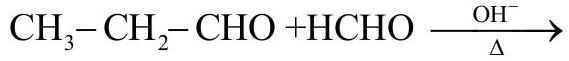
\includegraphics[max width=\textwidth, center]{2025_10_02_e189b9aa2c5cf056b6b6g-1}\\
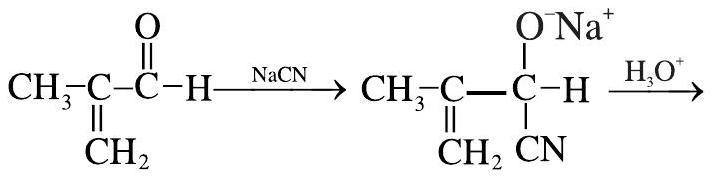
\includegraphics[max width=\textwidth, center]{2025_10_02_e189b9aa2c5cf056b6b6g-1(1)}\\
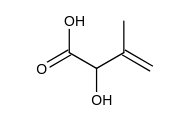
\includegraphics{smile-fd698bc90db7e6ce804e14dd993753ba48f78a5d}\\
\(( \pm)\)\\
Carboxylic acid will give \(\mathrm{CO}_{2}\) gas, with \(\mathrm{NaHCO}_{3}\) solution\\
34. The correct order of basicity of oxides of vanadium is\\
(1) \(\mathrm{V}_{2} \mathrm{O}_{3}>\mathrm{V}_{2} \mathrm{O}_{4}>\mathrm{V}_{2} \mathrm{O}_{5}\)\\
(2) \(\mathrm{V}_{2} \mathrm{O}_{3}>\mathrm{V}_{2} \mathrm{O}_{5}>\mathrm{V}_{2} \mathrm{O}_{4}\)\\
(3) \(\mathrm{V}_{2} \mathrm{O}_{5}>\mathrm{V}_{2} \mathrm{O}_{4}>\mathrm{V}_{2} \mathrm{O}_{3}\)\\
(4) \(\mathrm{V}_{2} \mathrm{O}_{4}>\mathrm{V}_{2} \mathrm{O}_{3}>\mathrm{V}_{2} \mathrm{O}_{5}\)

Official Ans. by NTA (1)\\
Allen Ans. (1)\\
Sol. With increase in \% of oxygen acidic nature of oxide of an element increase and basic nature decreases\\
35. When \(\mathrm{Cu}^{2+}\) ion is treated with KI, a white precipitate, \(X\) appears in solution. The solution is titrated with sodium thiosulphate, the compound Y is formed. X and Y respectively are\\
(1) \(\mathrm{X}=\mathrm{Cu}_{2} \mathrm{I}_{2} \mathrm{Y}=\mathrm{Na}_{2} \mathrm{~S}_{4} \mathrm{O}_{5}\)\\
(2) \(X=\mathrm{Cu}_{2} \mathrm{I}_{2} \mathrm{Y}=\mathrm{Na}_{2} \mathrm{~S}_{4} \mathrm{O}_{6}\)\\
(3) \(\mathrm{X}=\mathrm{CuI}_{2} \mathrm{Y}=\mathrm{Na}_{2} \mathrm{~S}_{4} \mathrm{O}_{3}\)\\
(4) \(\mathrm{X}=\mathrm{CuI}_{2} \mathrm{Y}=\mathrm{Na}_{2} \mathrm{~S}_{4} \mathrm{O}_{6}\)

Official Ans. by NTA (2)\\
Allen Ans. (2)\\
Sol.\\
\(\mathrm{Cu}^{2+}+2 \mathrm{KI} \longrightarrow \underset{\text { Unstable }}{\mathrm{CuI}_{2}} \downarrow+2 \mathrm{~K}^{+}\)\\
\(\mathrm{I}^{-}\)is strong R.A it reduces \(\mathrm{Cu}^{2+}\) to \(\mathrm{Cu}^{+}\)\\
\(2 \mathrm{CuI}_{2} \longrightarrow \underset{(\text { White })^{\prime} \mathrm{X}^{\prime}}{\mathrm{Cu}_{2} \mathrm{I}_{2}} \downarrow+\mathrm{I}_{2}\)\\
\(\mathrm{KI}+\mathrm{I}_{2} \longrightarrow \mathrm{~K}^{+} \mathrm{I}_{3}^{-}\)(Brown solution)\\
\(\mathrm{I}_{3}^{-} \rightleftharpoons \mathrm{I}_{2}+\mathrm{I}^{-}\)\\
\(\mathrm{KI}_{3}+\mathrm{Na}_{2} \mathrm{~S}_{2} \mathrm{O}_{3} \rightarrow \mathrm{KI}+\underset{(\mathrm{Y})}{\mathrm{Na}_{2} \mathrm{~S}_{4} \mathrm{O}_{6}}\)\\
36.\\
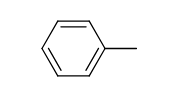
\includegraphics{smile-5eb24c2d8a39c514f31f1cc3e82f185790fd16d7}\\
\(\mathrm{NO}_{2}\)

\[
\xrightarrow[\mathrm{C}_{2} \mathrm{H}_{5} \mathrm{OH}]{\mathrm{H}_{2} / \mathrm{Pd}}[\mathrm{~A}] \xrightarrow[\text { Pyridine }]{\left(\mathrm{CH}_{3} \mathrm{CO}\right)_{2} \mathrm{O}}[\mathrm{~B}]
\]

(1)\\
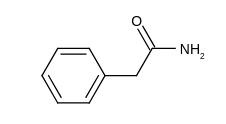
\includegraphics{smile-db37d5b7cd8dbaa70b7fe9fd2e8b876c055ee9f1}\\
(2)\\
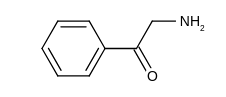
\includegraphics{smile-37fdccc21030344a582be8d48cab0dba418dffbd}\\
(3)\\
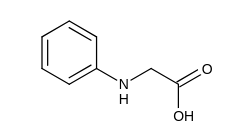
\includegraphics{smile-15db534f7327e0d5431eee834dd513b12312e0ee}\\
(4)\\
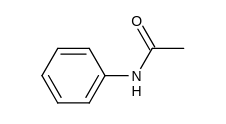
\includegraphics{smile-c545f174638d6a2bdd2cdb149c6d2ed8460112f9}

Official Ans. by NTA (4)\\
Allen Ans. (4)\\
Sol.\\
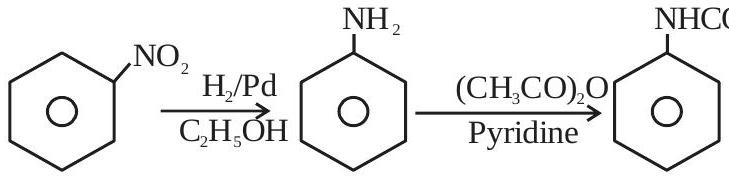
\includegraphics[max width=\textwidth, center]{2025_10_02_e189b9aa2c5cf056b6b6g-2}\\
37. Cobalt chloride when dissolved in water forms pink colored complex X which has octahedral geometry. This solution on treating with cone HCl forms deep blue complex, Y which has a Z geometry. \(\mathrm{X}, \mathrm{Y}\) and Z , respectively, are\\
(1) \(\mathrm{X}=\left[\mathrm{Co}\left(\mathrm{H}_{2} \mathrm{O}\right)_{6}\right]^{2+}, \mathrm{Y}=\left[\mathrm{CoCl}_{4}\right]^{2-}, \mathrm{Z}=\) Tetrahedral\\
(2) \(\mathrm{X}=\left[\mathrm{Co}\left(\mathrm{H}_{2} \mathrm{O}_{6}\right)\right]^{2+}, \mathrm{Y}=\left[\mathrm{CoCl}_{6}\right]^{3-}, \mathrm{Z}=\) Octahedral\\
(3) \(\mathrm{X}=\left[\mathrm{Co}\left(\mathrm{H}_{2} \mathrm{O}\right)_{6}\right]^{3+}, \mathrm{Y}=\left[\mathrm{CoCl}_{6}\right]^{3-}, \mathrm{Z}=\) Octahedral\\
(4) \(\mathrm{X}=\left[\mathrm{Co}\left(\mathrm{H}_{2} \mathrm{O}\right)_{4} \mathrm{Cl}_{2}\right]^{+}, \mathrm{Y}=\left[\mathrm{CoCl}_{4}\right]^{2-}, \mathrm{Z}=\) Tetrahedral

Official Ans. by NTA (1)\\
Allen Ans. (1)\\
Sol.\\
\(\mathrm{CoCl}_{2}+6 \mathrm{H}_{2} \mathrm{O} \longrightarrow\left[\mathrm{Co}\left(\mathrm{H}_{2} \mathrm{O}\right)_{6}\right] \mathrm{Cl}_{2}\)\\
Pink(X)\\
octahedral\\
\(\downarrow+\mathrm{HCl}\) (conc.)\\
\(\left[\mathrm{CoCl}_{4}\right]^{2-}\)\\
(Y)Blue solution\\
(Z)Tetrahedral\\
38. Identify \(\mathrm{X}, \mathrm{Y}\) and Z in the following reaction. (Equation not balanced)\\
\(\mathrm{Cl} \dot{\mathrm{O}}+\mathrm{NO}_{2} \rightarrow \underline{\mathrm{X}} \xrightarrow{\mathrm{H}_{2} \mathrm{O}} \underline{\mathrm{Y}}+\underline{\mathrm{Z}}\)\\
(1) \(\mathrm{X}=\mathrm{ClONO}_{2}, \mathrm{Y}=\mathrm{HOCl}, \mathrm{Z}=\mathrm{NO}_{2}\)\\
(2) \(\mathrm{X}=\mathrm{ClNO}_{2}, \mathrm{Y}=\mathrm{HCl}, \mathrm{Z}=\mathrm{HNO}_{3}\)\\
(3) \(\mathrm{X}=\mathrm{ClONO}_{2}, \mathrm{Y}=\mathrm{HOCl}, \mathrm{Z}=\mathrm{HNO}_{3}\)\\
(4) \(\mathrm{X}=\mathrm{ClNO}_{3}, \mathrm{Y}=\mathrm{Cl}_{2}, \mathrm{Z}=\mathrm{NO}_{2}\)

Official Ans. by NTA (3)\\
Allen Ans. (3)\\
Sol. \(\quad \mathrm{ClO}+\mathrm{NO}_{2} \longrightarrow \underset{(\mathrm{X})}{\mathrm{ClONO}} \xrightarrow{+\mathrm{H}_{2} \mathrm{O}} \underset{(\mathrm{Y})}{\mathrm{HOCl}}+\underset{(\mathrm{Z})}{\mathrm{HNO}_{3}}\)\\
39. The correct order of melting point of dichlorobenzenes is\\
(1)\\
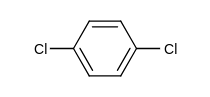
\includegraphics{smile-f872fca38963d27b33094fbbbfa08dd49204121f}\\
\(>\)\\
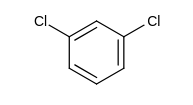
\includegraphics{smile-27f94bf22a4720515798de0a97a5388fbdc8befb}\\
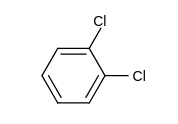
\includegraphics{smile-6bab4884159b801c6b5a03d7b981394c86b9170c}\\
(2)\\
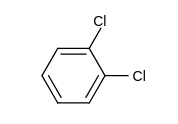
\includegraphics{smile-b97a614a1fcc58e833b49ef98b44c64d19492386}\\
\(>\)\\
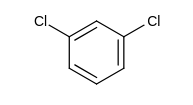
\includegraphics{smile-c37cc52f4c0c743015b0809585746648b91e1e4f}\\
\(>\)\\
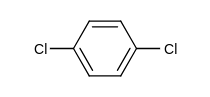
\includegraphics{smile-ecc9d7430ad373b85fd2b7c099326eceebbb051c}\\
(3)\\
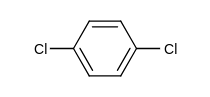
\includegraphics{smile-149b290a73a5de682badd45e3b1382bf8ed1b80f}\\
\(>\)\\
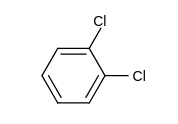
\includegraphics{smile-a878544e719910f4a23fd6ee02c243956d151914}\\
(4)\\
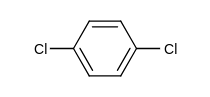
\includegraphics{smile-82286d6e4b478adc8e9bb0e630580cc5ff808ad5}\\
\(>\)\\
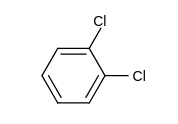
\includegraphics{smile-34eecfe6a8a8577aff5169738d9ad5be41eeabf6}\\
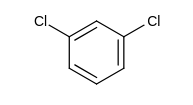
\includegraphics{smile-654e323693dda5e718dadb148136aec7c5b1dabb}

Official Ans. by NTA (4)\\
Allen Ans. (4)\\
Sol.\\
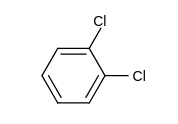
\includegraphics{smile-2d8472bce3871b16a612fb6368e189b8ac25365a}

b.p / K\\
m.p / K\\
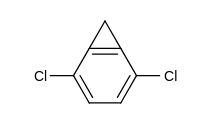
\includegraphics{smile-57507b5efe31782915b72ae9be55164ce6a8c4d7}

More Symmetrical \& better Crystal fitting\\
M.P a Packing efficiency\\
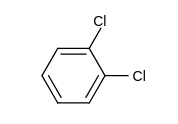
\includegraphics{smile-41b8d537df38895773f5240f63ee40d392e597eb}\\
\(\Rightarrow \mu_{\text {max }}\)\\
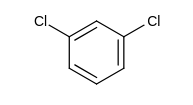
\includegraphics{smile-896b1bf5a2a5aa40140fd32899a9b550538d3ada}\\
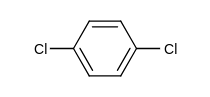
\includegraphics{smile-6c0ba2f3393653179997b107945acd5bd4792034}

448\\
323\\
40. A protein ' \(X\) ' with molecular weight of \(70,000 \mathrm{u}\), on hydrolysis gives amino acids. One of these amino acid is\\
(1)\\
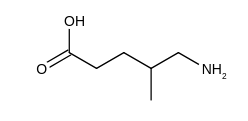
\includegraphics{smile-79a5e0ab2483cf39e419960f6303b495a8efd22d}\\
(2)\\
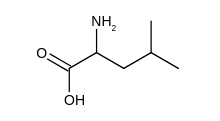
\includegraphics{smile-b0c5ced56a11062d0219aac1e251e0011062b888}\\
(3)\\
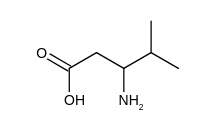
\includegraphics{smile-76ad6181fffa9acd324007ea45e1f74956e792d9}\\
(4)\\
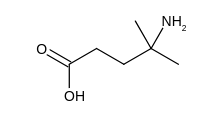
\includegraphics{smile-659becae5e64b369ea616ee2ec2ac9900cc05cc7}

Official Ans. by NTA (2)\\
Allen Ans. (2)\\
Sol. Only in option (2) \(\alpha\)-Amino acid is given all the other options are not \(\alpha\)-Amino acids.\\
41. Which transition in the hydrogen spectrum would have the same wavelength as the Balmer type transition from \(n=4\) to \(n=2\) of \(\mathrm{He}^{+}\)spectrum\\
(1) \(n=2\) to \(n=1\)\\
(2) \(n=1\) to \(n=3\)\\
(3) \(n=1\) to \(n=2\)\\
(4) \(n=3\) to \(n=4\)

Official Ans. by NTA (1)\\
Allen Ans. (1)\\
Sol. \(\mathrm{He}^{+}\)ion :\\
\(\frac{1}{\lambda(\mathrm{H})}=\mathrm{R}(1)^{2}\left[\frac{1}{\mathrm{n}_{1}^{2}}-\frac{1}{\mathrm{n}_{2}^{2}}\right]\)\\
\(\frac{1}{\lambda\left(\mathrm{He}^{+}\right)}=\mathrm{R}(2)^{2}\left[\frac{1}{2^{2}}-\frac{1}{4^{2}}\right]\)\\
Given \(\lambda(\mathrm{H})=\lambda\left(\mathrm{He}^{+}\right)\)\\
\(\mathrm{R}(1)^{2}\left[\frac{1}{\mathrm{n}_{1}^{2}}-\frac{1}{\mathrm{n}_{2}^{2}}\right]=\mathrm{R}(4)\left[\frac{1}{2^{2}}-\frac{1}{4^{2}}\right]\)\\
\(\frac{1}{\mathrm{n}_{1}^{2}}-\frac{1}{\mathrm{n}_{2}^{2}}=\frac{1}{1^{2}}-\frac{1}{2^{2}}\)\\
On comparing \(\mathrm{n}_{1}=1 \& \mathrm{n}_{2}=2\)\\
Ans. 1\\
42. Match items of column I and II

\begin{center}
\begin{tabular}{|l|l|}
\hline
Column I (Mixture of compounds) & Column II (Separation Technique) \\
\hline
A. \(\mathrm{H}_{2} \mathrm{O} / \mathrm{CH}_{2} \mathrm{Cl}_{2}\) & i. Crystallization \\
\hline
B. 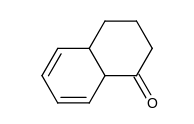
\includegraphics{smile-fa7bf8395e0f8c8d06dae02989b363143130d8ce} & ii. Differential solvent extraction \\
\hline
C. Kerosene/Naphthalene & iii. Column chromatography \\
\hline
D. \(\mathrm{C}_{6} \mathrm{H}_{12} \mathrm{O}_{6} / \mathrm{NaCl}\) & iv. Fractional Distillation \\
\hline
\end{tabular}
\end{center}

Correct match is :\\
(1) A-(iii), B-(iv), C-(ii), D-(i)\\
(2) A-(i), B-(iii), C-(ii), D-(iv)\\
(3) A-(ii), B-(iii), C-(iv), D-(i)\\
(4) A-(ii), B-(iv), C-(i), D-(iii)

Official Ans. by NTA (3)\\
Allen Ans. (3)\\
Sol. A. \(\mathrm{H}_{2} \mathrm{O} / \mathrm{CH}_{2} \mathrm{Cl}_{2} \rightarrow \mathrm{ii}, \mathrm{CH}_{2} \mathrm{Cl}_{2}>\mathrm{H}_{2} \mathrm{O}\) (density) so they can be separated by differential solvent extraction.\\
B.\\
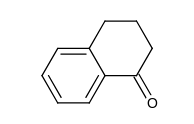
\includegraphics{smile-ac60576f6246db3f347fa354c9df6493ed5d4df6}\\
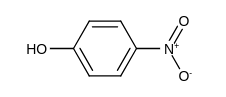
\includegraphics{smile-227d07bad614a7b6cadb43412e8a8305167423a2}\\
iii. column\\
chromatography

Due to H-bonding in\\
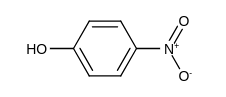
\includegraphics{smile-d66fafa6f7fefe4660a93ab4ffb600b8d629ecfe}\\
it can be separated\\
from\\
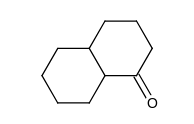
\includegraphics{smile-b617193cc47e1a66ae95515fe7775ba09427eeba}\\
by column chromatography.\\
C. Kerosene / Naphthalene \(\rightarrow\) iv. Fractional distillation.

Due to different B.P. of kerosene and Naphthalene it can be separated by fractional distillation.\\
D. \(\mathrm{C}_{6} \mathrm{H}_{12} \mathrm{O}_{6} / \mathrm{NaCl} \rightarrow \mathrm{i}\). Crystallization.

NaCl (ionic compound) can be crystallized.\\
43. The correct increasing order of the ionic radii is\\
(1) \(\mathrm{Cl}^{-}<\mathrm{Ca}^{2+}<\mathrm{K}^{+}<\mathrm{S}^{2-}\)\\
(2) \(\mathrm{K}^{+}<\mathrm{S}^{2-}<\mathrm{Ca}^{2+}<\mathrm{Cl}^{-}\)\\
(3) \(\mathrm{S}^{2-}<\mathrm{Cl}^{-}<\mathrm{Ca}^{2+}<\mathrm{K}^{+}\)\\
(4) \(\mathrm{Ca}^{2+}<\mathrm{K}^{+}<\mathrm{Cl}^{-}<\mathrm{S}^{2-}\)

Official Ans. by NTA (4)\\
Allen Ans. (4)\\
Sol. In isoelectronic species size \(\propto \frac{1}{\mathrm{Z}}\)

\[
\begin{array}{rlrrl} 
& \mathrm{Ca}^{2+}<\mathrm{K}^{+}<\mathrm{Cl}^{-}<\mathrm{S}^{2-}: \text { Size } \\
\mathrm{Z}: & 20 & 19 & 17 & 18
\end{array}
\]

\begin{enumerate}
  \setcounter{enumi}{43}
  \item \(\mathrm{H}_{2} \mathrm{O}_{2}\) acts as a reducing agent in\\
(1) \(2 \mathrm{NaOCl}+\mathrm{H}_{2} \mathrm{O}_{2} \rightarrow 2 \mathrm{NaCl}+\mathrm{H}_{2} \mathrm{O}+\mathrm{O}_{2}\)\\
(2) \(2 \mathrm{Fe}^{2+}+2 \mathrm{H}^{+}+\mathrm{H}_{2} \mathrm{O}_{2} \rightarrow 2 \mathrm{Fe}^{3+}+2 \mathrm{H}_{2} \mathrm{O}\)\\
(3) \(\mathrm{Mn}^{2+}+2 \mathrm{H}_{2} \mathrm{O}_{2} \rightarrow \mathrm{MnO}_{2}+2 \mathrm{H}_{2} \mathrm{O}\)\\
(4) \(\mathrm{Na}_{2} \mathrm{~S}+4 \mathrm{H}_{2} \mathrm{O}_{2} \rightarrow \mathrm{Na}_{2} \mathrm{SO}_{4}+4 \mathrm{H}_{2} \mathrm{O}\)
\end{enumerate}

Official Ans. by NTA (1)\\
Allen Ans. (1)\\
Sol. \(\underset{+1}{\mathrm{NaOCl}}+\underset{+}{\mathrm{H}_{2} \mathrm{O}_{2}} \longrightarrow \underset{(-1)}{-1} \underset{+}{2 \mathrm{NaCl}}+\underset{+}{\mathrm{H}_{2} \mathrm{O}}+\underset{+}{\mathrm{O}_{2}}\)\\
45. Which of the following artificial sweeteners has the highest sweetness value in comparison to cane sugar?\\
(1) Aspartame\\
(2) Sucralose\\
(3) Alitame\\
(4) Saccharin

Official Ans. by NTA (3)\\
Allen Ans. (3)\\
Sol. Sweetness value order wrt cane sugar\\
Alitame \(>\) Sucralose \(>\) Saccharin \(>\) Aspartame\\
46. Match List I with List II

\begin{center}
\begin{tabular}{|l|l|}
\hline
List I & List II \\
\hline
A. \(\mathrm{XeF}_{4}\) & I.See - saw \\
\hline
B. \(\mathrm{SF}_{4}\) & II. Square planar \\
\hline
C. \(\mathrm{NH}_{4}^{+}\) & III. Bent T - shaped \\
\hline
D. \(\mathrm{BrF}_{3}\) & IV. Tetrahedral \\
\hline
\end{tabular}
\end{center}

Choose the correct answer from the options given below :\\
(1) A-IV, B-III, C-II, D-I\\
(2) A-II, B-I, C-III, D-IV\\
(3) A-IV, B-I, C-II, D-III\\
(4) A-II, B-I, C-IV, D-III

Official Ans. by NTA (4)\\
Allen Ans. (4)\\
Sol.\\
(A)\\
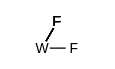
\includegraphics{smile-7c2e4d0d45614351b9ab9debf457d3f062578191}

Square planer\\
(B) \(\mathrm{SF}_{4}\)\\
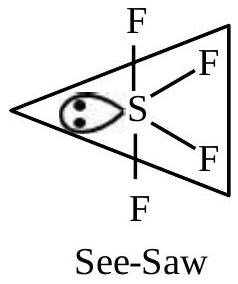
\includegraphics[max width=\textwidth, center]{2025_10_02_e189b9aa2c5cf056b6b6g-4}\\
(C) \(\mathrm{NH}_{4}^{+}\)\\
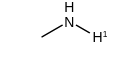
\includegraphics{smile-d060142afdf03021cf82e65f98c7aa7aaa9dce75}

Tetrahedral\\
(D) \(\mathrm{Br} \mathrm{F}_{3}\)\\
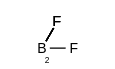
\includegraphics{smile-8bf7b2f769ef2fec65a53d3934f835e6442246c2}

Bent T- Shaped\\
47. Choose the correct set of reagents for the following conversion\\
trans \(\left(\mathrm{Ph}-\mathrm{CH}=\mathrm{CH}-\mathrm{CH}_{3}\right) \rightarrow\) cis \(\left(\mathrm{Ph}-\mathrm{CH}=\mathrm{CH}-\mathrm{CH}_{3}\right)\)\\
(1) \(\mathrm{Br}_{2}\), alc \(\mathrm{KOH}, \mathrm{NaNH}_{2}, \mathrm{Na}\left(\mathrm{Liq} \mathrm{NH} \mathrm{H}_{3}\right)\)\\
(2) \(\mathrm{Br}_{2}\), alc \(\mathrm{KOH}, \mathrm{NaNH}_{2}, \mathrm{H}_{2}\) Lindlar Catalyst\\
(3) \(\mathrm{Br}_{2}, \mathrm{aq} \mathrm{KOH}, \mathrm{NaNH}_{2}, \mathrm{H}_{2}\) Lindlar Catalyst\\
(4) \(\mathrm{Br}_{2}, \mathrm{aq} \mathrm{KOH}, \mathrm{NaNH}_{2}, \mathrm{Na}\left(\mathrm{Liq} \mathrm{NH}_{3}\right)\)

Official Ans. by NTA (2)\\
Allen Ans. (2)\\
Sol.\\
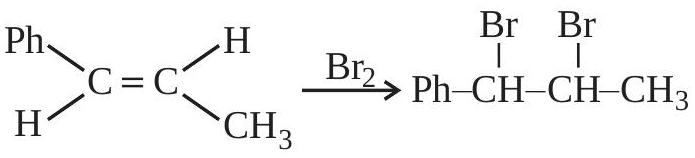
\includegraphics[max width=\textwidth, center]{2025_10_02_e189b9aa2c5cf056b6b6g-5(3)}\\
(1) Alc. KOH\\
(2) \(\mathrm{NaNH}_{2}\)\\
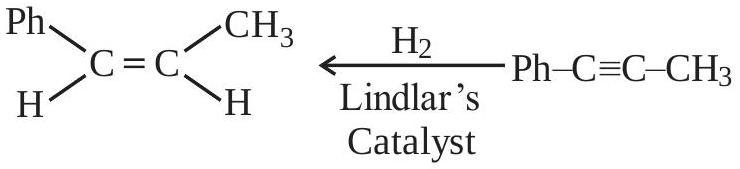
\includegraphics[max width=\textwidth, center]{2025_10_02_e189b9aa2c5cf056b6b6g-5}\\
48. Adding surfactants in non polar solvent, the micelles structure will look like\\
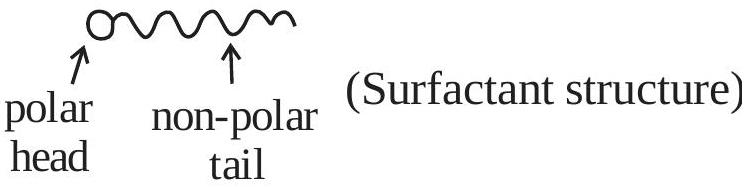
\includegraphics[max width=\textwidth, center]{2025_10_02_e189b9aa2c5cf056b6b6g-5(2)}\\
(a)\\
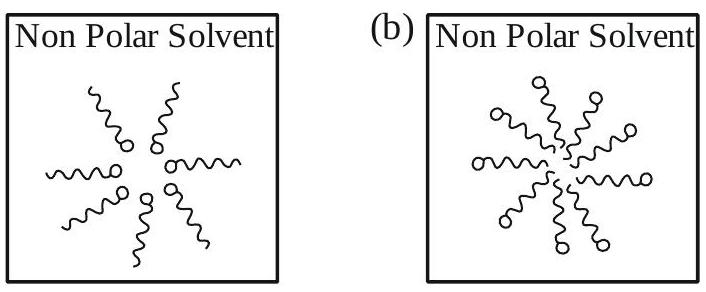
\includegraphics[max width=\textwidth, center]{2025_10_02_e189b9aa2c5cf056b6b6g-5(4)}\\
(c)

\begin{center}
\begin{tabular}{|l|}
\hline
Non Polar Solvent \\
\hline
\( \begin{aligned} & \} \\ & \} \\ & \} \\ & \} \end{aligned} \) \\
\hline
\end{tabular}
\end{center}

(d) Non Polar Solvent\\
(1) b\\
(2) c\\
(3) a\\
(4) d

Official Ans. by NTA (3)\\
Allen Ans. (3)\\
Sol. Non-Polar tail towards non-polar solvent\\
Ans. 3\\
49. An organic compound 'A' with empirical formula \(\mathrm{C}_{6} \mathrm{H}_{6} \mathrm{O}\) gives sooty flame on burning. Its reaction with bromine solution in low polarity solvent results in high yield of B . B is\\
(1)\\
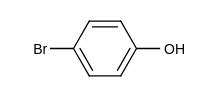
\includegraphics{smile-8252d745ede9d8cb2fafb281a5df775b4b1f092b}\\
(2)\\
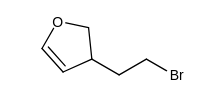
\includegraphics{smile-75eef1803918471bcfffd4ff50a4c2ae2f9ff4b0}\\
(3)\\
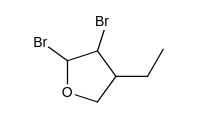
\includegraphics{smile-f4de795c2fdec99b6fe9a7484b717c6df647c346}\\
(4)\\
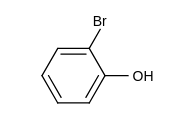
\includegraphics{smile-3273a963f1eb51a41ba70dc1f1408332a4e45ce1}

Official Ans. by NTA (1)\\
Allen Ans. (1)\\
Sol. Aromatic compounds burns with sooty flame\\
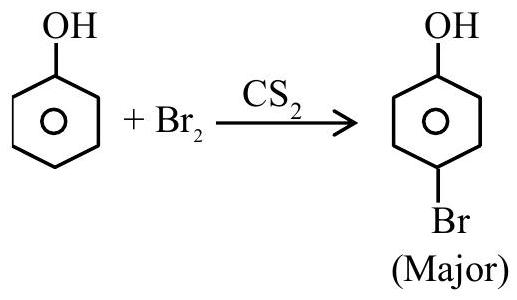
\includegraphics[max width=\textwidth, center]{2025_10_02_e189b9aa2c5cf056b6b6g-5(1)}\\
50. Which one of the following statements is correct for electrolysis of brine solution?\\
(1) \(\mathrm{Cl}_{2}\) is formed at cathode\\
(2) \(\mathrm{O}_{2}\) is formed at cathode\\
(3) \(\mathrm{H}_{2}\) is formed at anode\\
(4) \(\mathrm{OH}^{-}\)is formed at cathode

Official Ans. by NTA (4)\\
Allen Ans. (4)\\
Sol. Electrolysis of brine solution\\
NaCl (aq.) \(\longrightarrow \mathrm{Na}_{\text {(aq) }}^{+}+\mathrm{Cl}_{\text {(aq) }}^{+}\)\\
At anode : \(2 \mathrm{Cl}_{\text {(aq.) }}^{+} \longrightarrow \underset{\text { (Major) }}{\mathrm{Cl}_{2}(\mathrm{~g})}+2 \mathrm{e}^{-}\)\\
\(2 \mathrm{H}_{2} \mathrm{O}_{(\ell)} \longrightarrow \underset{\text { Minor }}{\mathrm{O}_{2(\mathrm{~g})}}+4 \mathrm{H}_{(\mathrm{aq})}^{+}+4 \mathrm{e}^{-}\)\\
At Cathode : \(2 \mathrm{H}_{2} \mathrm{O}_{(\ell)}+2 \mathrm{e}^{-} \longrightarrow \mathrm{H}_{2(\mathrm{~g})} \uparrow+2 \mathrm{OH}_{(\mathrm{aq})}^{-}\)\\
\(2 \mathrm{Na}^{+}+2 \mathrm{OH}^{-} \longrightarrow 2 \mathrm{NaOH}\)

\section*{SECTION-B}
\begin{enumerate}
  \setcounter{enumi}{50}
  \item The logarithm of equilibrium constant for the reaction \(\quad \mathrm{Pd}^{2+}+4 \mathrm{Cl}^{-} \rightleftharpoons \mathrm{PdCl}_{4}^{2-} \quad\) is \(\_\_\_\_\)\\
(Nearest integer)\\
Given: \(\frac{2.303 \mathrm{RT}}{\mathrm{F}}=0.06 \mathrm{~V}\)\\
\(\mathrm{Pd}_{(\mathrm{aq})}^{2+}+2 \mathrm{e}^{-} \rightleftharpoons \mathrm{Pd}(\mathrm{s}) \quad \mathrm{E}^{\mathrm{o}}=0.83 \mathrm{~V}\)\\
\(\mathrm{PdCl}_{4}^{2-}(\mathrm{aq})+2 \mathrm{e}^{-} \rightleftharpoons \mathrm{Pd}(\mathrm{s})+4 \mathrm{Cl}^{-}(\mathrm{aq})\)\\
\(\mathrm{E}^{\circ}=0.65 \mathrm{~V}\)\\
Official Ans. by NTA (6)\\
Allen Ans. (6)\\
Sol. \(\Delta \mathrm{G}^{\mathrm{o}}=-\mathrm{RT} \ell \mathrm{nK}\)\\
\(-n F E_{\text {cell }}^{o}=-R T \times 2.303\left(\log _{10} K\right)\)\\
\(\frac{\mathrm{E}_{\text {Cell }}^{\mathrm{o}}}{0.06} \times \mathrm{n}=\log \mathrm{K}\)\\
\(\mathrm{Pd}^{+2}\) (aq.) \(+\not \mathcal{L}^{-} \rightleftharpoons \mathrm{Pd}(\mathrm{s}), \mathrm{E}^{\mathrm{o}}{ }_{\text {cat,red }}=0.83\)\\
\(\mathrm{Pd}(\mathrm{s})+4 \mathrm{Cl}^{-}(\mathrm{aq}.) \rightleftharpoons \mathrm{PdCl}_{4}^{2-},(\mathrm{aq})+2 \mathrm{e}^{-}, \mathrm{E}_{\text {Anode,Oxid }}^{\circ}=0.65\)\\
Net Reaction \(\rightarrow \mathrm{Pd}^{2+}\) (aq.) \(+4 \mathrm{Cl}^{-}\)(aq.) \(\rightleftharpoons \mathrm{PdCl}_{4}{ }^{2-}\) (aq.)\\
\(\mathrm{E}_{\text {cell }}^{\mathrm{o}}=\mathrm{E}_{{ }_{\text {cat }, \text { red }}}^{\mathrm{o}}-\mathrm{E}_{\text {Anode,Oxid }}^{\mathrm{o}}\)\\
\(\mathrm{E}_{\text {cell }}^{\mathrm{o}}=0.83-0.65\)\\
\(\mathrm{E}_{\text {cell }}^{\mathrm{o}}=0.18\)
\end{enumerate}

Also \(\mathrm{n}=2\)

Using equation (1), (2) \& (3)\\
\(\log \mathrm{K}=6\)\\
52. \(\mathrm{A} \rightarrow \mathrm{B}\)

The rate constants of the above reaction at 200 K and 300 K are \(0.03 \mathrm{~min}^{-1}\) and \(0.05 \mathrm{~min}^{-1}\) respectively. The activation energy for the reaction is \(\_\_\_\_\) J (Nearest integer)\\
(Given : In \(10=2.3\)\\
\(\mathrm{R}=8.3 \mathrm{~J} \mathrm{~K}^{-1} \mathrm{~mol}^{-1}\)\\
\(\log 5=0.70\)\\
\(\log 3=0.48\)\\
\(\log 2=0.30\)\\
Official Ans. by NTA (2520)\\
Allen Ans. (2520)\\
Sol.\\
\(\log \frac{\mathrm{K}_{300}}{\mathrm{~K}_{200}}=\frac{\mathrm{E}_{\mathrm{a}}}{2.3 \times 8.314}\left(\frac{1}{\mathrm{~T}_{1}}-\frac{1}{\mathrm{~T}_{2}}\right)\)\\
\(\log \frac{0.05}{0.03}=\frac{\mathrm{Ea}}{2.305 \times 8.314} \times\left[\frac{1}{200}-\frac{1}{300}\right]\)\\
\(\mathrm{E}_{\mathrm{a}}=2519.88 \mathrm{~J} \Rightarrow \mathrm{E}_{\mathrm{a}}=2520 \mathrm{~J}\)\\
53. The enthalpy change for the conversion of \(\frac{1}{2} \mathrm{Cl}_{2}(\mathrm{~g})\) to \(\mathrm{Cl}^{-}(\mathrm{aq})\) is \((-)\) \(\_\_\_\_\)\\
\(\mathrm{kJ} \mathrm{mol}^{-1}\) (Nearest integer)\\
Given : \(\Delta_{\text {dis }} \mathrm{H}_{\mathrm{Cl}_{2(\mathrm{~g})}^{\mathrm{o}}}=240 \mathrm{kJmol}^{-1}\).\\
\(\Delta_{\mathrm{eg}} \mathrm{H}_{\mathrm{Cl}_{(\mathrm{g})}}^{\mathrm{o}}=-350 \mathrm{kJmol}^{-1}\),\\
\(\Delta_{\text {hyd }} \mathrm{H}_{\mathrm{Cl}_{(\mathrm{g})}^{-}}=-380 \mathrm{kJmol}^{-1}\)\\
Official Ans. by NTA (610)\\
Allen Ans. (610)\\
Sol. \(\quad \frac{1}{2} \mathrm{Cl}_{2(\mathrm{~g})} \rightarrow \mathrm{Cl}_{(\mathrm{g})} \rightarrow \mathrm{Cl}_{(\mathrm{g})}^{-} \rightarrow \mathrm{Cl}_{(\text {aq. })}^{-}\)\\
\(\Delta \mathrm{H}^{\mathrm{o}}=\frac{1}{2} \times 240+(-350)+(-380)\)\\
\(=-610\) ans.\\
54. On complete combustion, 0.492 g of an organic compound gave 0.792 g of \(\mathrm{CO}_{2}\).

The \% of carbon in the organic compound is \(\_\_\_\_\)\\
(Nearest integer)\\
Official Ans. by NTA (44)\\
Allen Ans. (44)\\
Sol. weight of C in \(0.792 \mathrm{gm} \mathrm{CO}_{2}\)

\[
\begin{aligned}
& =\frac{12}{44} \times 0.792=0.216 \\
& \% \text { of } \mathrm{C} \text { in compound }=\frac{0.216}{0.492} \times 100 \\
& =43.90 \%
\end{aligned}
\]

Ans : 44\\
55. At \(27^{\circ} \mathrm{C}\), a solution containing 2.5 g of solute in 250.0 mL of solution exerts an osmotic pressure of 400 Pa . The molar mass of the solute is \(\_\_\_\_\) g \(\mathrm{mol}^{-1}\) (Nearest integer)\\
(Given : \(\mathrm{R}=0.083 \mathrm{~L}\) bar \(\mathrm{K}^{-1} \mathrm{~mol}^{-1}\) )\\
Official Ans. by NTA (62250)\\
Allen Ans. (62250)\\
Sol. : \(\pi=\) CRT\\
\(\frac{400 \mathrm{~Pa}}{10^{5}}=\frac{\frac{2.5 \mathrm{~g}}{\mathrm{M}_{\mathrm{o}}}}{250 / 1000 \mathrm{~L}} \times 0.83 \frac{\mathrm{~L}-\text { bar }}{\text { K.mol }} \times 300 \mathrm{~K}\)\\
\(\mathrm{M}_{\mathrm{o}}=62250\)\\
56. Zinc reacts with hydrochloric acid to give hydrogen and zinc chloride. The volume of hydrogen gas produced at STP from the reaction of 11.5 g of zinc with excess HCl is \(\_\_\_\_\) L (Nearest integer)\\
(Given : Molar mass of Zn is \(65.4 \mathrm{~g} \mathrm{~mol}^{-1}\) and Molar volume of \(\mathrm{H}_{2}\) at \(\mathrm{STP}=22.7 \mathrm{~L}\) )\\
Official Ans. by NTA (4)\\
Allen Ans. ( 4)\\
Sol. \(\quad \mathrm{Zn}+2 \mathrm{HCl} \rightarrow \mathrm{ZnCl}_{2}+\mathrm{H}_{2} \uparrow\)\\
Moles of Zn used \(=\frac{11.5}{65.4}=\) Moles of \(\mathrm{H}_{2}\) evolved\\
Volume of \(\mathrm{H}_{2}=\frac{11.5}{65.4} \times 22.7 \mathrm{~L}=3.99 \mathrm{~L}\)\\
Ans : 4\\
57. How many of the transformation given below would result in aromatic amines?\\
(1)\\
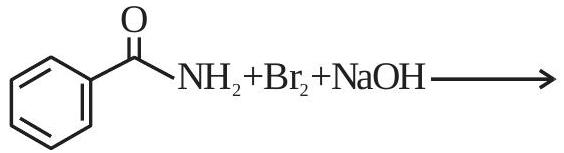
\includegraphics[max width=\textwidth, center]{2025_10_02_e189b9aa2c5cf056b6b6g-7(1)}\\
(2)\\
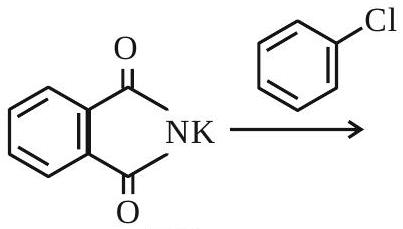
\includegraphics[max width=\textwidth, center]{2025_10_02_e189b9aa2c5cf056b6b6g-7(3)}\\
(3)\\
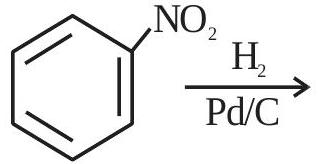
\includegraphics[max width=\textwidth, center]{2025_10_02_e189b9aa2c5cf056b6b6g-7}\\
(4)\\
\includegraphics[max width=\textwidth, center]{2025_10_02_e189b9aa2c5cf056b6b6g-7(2)}

Official Ans. by NTA (3)\\
Allen Ans. (3)\\
Sol. Product in the given reactions are as follow-\\
1.\\
\includegraphics{smile-e03a58f5a921c2b40a9be6c405169b2bd22b8f0c}\\
2. No reactions will be observed as in Gabriel phthalimide synthesis\\
\includegraphics{smile-8513654ed542bd219801d15ae620ac156e9292e5}\\
is poor substrate for \(\mathrm{SN}^{2}\)\\
3.\\
\includegraphics{smile-47bebfb765409c22a02c6ab962d3272957113c5c}\\
4.\\
\includegraphics{smile-c02963e3b642135922b337af21aadd176af81346}\\
\(+\mathrm{CH}_{3} \mathrm{COOH}\)

Aromatic amines will he formed in 1, \(3 \& 4\) Ans : 3\\
58. For reaction : \(\mathrm{SO}_{2}(\mathrm{~g})+\frac{1}{2} \mathrm{O}_{2}(\mathrm{~g}) \rightleftharpoons \mathrm{SO}_{3}(\mathrm{~g})\)\\
\(\mathrm{K}_{\mathrm{P}}=2 \times 10^{12}\) at \(27^{\circ} \mathrm{C}\) and 1 atm pressure. The \(\mathrm{K}_{\mathrm{c}}\) for the same reaction is \(\_\_\_\_\) \(\times 10^{13}\). (Nearest integer)\\
(Given \(\mathrm{R}=0.082 \mathrm{~L} \mathrm{~atm} \mathrm{~K}^{-1} \mathrm{~mol}^{-1}\) )\\
Official Ans. by NTA (1)\\
Allen Ans. (1)\\
sol. \(\quad \mathrm{SO}_{2(\mathrm{~g})}+\frac{1}{2} \mathrm{O}_{2(\mathrm{~g})} \rightleftharpoons \mathrm{SO}_{3(\mathrm{~g})}\)\\
\(\mathrm{K}_{\mathrm{P}}=2 \times 10^{12}\) at 300 K\\
\(\mathrm{K}_{\mathrm{P}}=\mathrm{K}_{\mathrm{C}} \times(\mathrm{RT})^{\Delta \mathrm{n}_{\mathrm{g}}}\)\\
\(2 \times 10^{12}=\mathrm{K}_{\mathrm{c}} \times(0.082 \times 300)^{-1 / 2}\)\\
\(\mathrm{K}_{\mathrm{C}}=9.92 \times 10^{12}\)\\
\(\mathrm{K}_{\mathrm{C}}=0.992 \times 10^{13}\)\\
Ans. 1\\
59. The oxidation sate of phosphorus in hypophosphoric acid is + \(\_\_\_\_\)。\\
Official Ans. by NTA (4)\\
Allen Ans. (4)\\
Sol. \(\mathrm{H}_{4} \mathrm{P}_{2} \mathrm{O}_{6}\)\\
\includegraphics{smile-6195cf44e991b82938bd5565a5921eb5cb638171}\\
O.S. of P is +4\\
60. The total pressure of a mixture of non-reacting gases \(\mathrm{X}(0.6 \mathrm{~g})\) and \(\mathrm{Y}(0.45 \mathrm{~g})\) in a vessel is 740 mm of Hg . The partial pressure of the gas X is\\
\(\_\_\_\_\) mm of Hg. (Nearest Integer)\\
(Given : molar mass \(\mathrm{X}=20\) and \(\mathrm{Y}=45 \mathrm{~g} \mathrm{~mol}^{-1}\) )\\
Official Ans. by NTA (555)\\
Allen Ans. (555)\\
Sol. \(\mathrm{P}_{\mathrm{X}}=\chi_{\mathrm{X}} \mathrm{P}_{\mathrm{T}}\)\\
\(=\frac{\frac{0.6}{20}}{\frac{0.6}{20}+\frac{0.45}{45}} \times 740\)\\
\(\mathrm{P}_{\mathrm{X}}=555 \mathrm{~mm} \mathrm{Hg}\)


\end{document}